\documentclass[12pt, letterpaper]{../assignment}
\usepackage{graphicx}
\usepackage{courier}
\usepackage{minted}
\usepackage{amsmath}
\usepackage{commath}
\usepackage{amssymb}
\usepackage{amsfonts} 
\usepackage{cancel}
\usepackage{enumitem}
\usepackage{array}

\usepackage{tikz}
\usetikzlibrary{shapes,arrows,positioning}

\usemintedstyle{monokai}
\oddsidemargin = 0pt
\exercisesheet{Module 14}{Practice Assignment}
\student{Austin Barrilleaux}
\courselabel{EN 525.609}
\semester{Fall 2023}
\usepackage[backend=bibtex,style=numeric,sorting=none]{biblatex}
\bibliography{reference}
\usepackage{color}
\definecolor{light-gray}{rgb}{0.2,0.2,0.2}
\setminted{bgcolor=light-gray}
\setlength{\parindent}{0pt}

\makeatletter
\patchcmd{\minted@colorbg}{\noindent}{\medskip\noindent}{}{}
\apptocmd{\endminted@colorbg}{\par\medskip}{}{}
\makeatother

\begin{document}
\subsection*{Problem 1}

\subsubsection*{Solve the following 9th Edition textbook problems:\\
\begin{itemize}
    \item 10-18 (a,c,f)
    \item 10-59 (a)
\end{itemize}}

\subsubsection*{(10-18) Check the contro1ihi1ity of the following systems:}

\subsubsection*{(a) \ \ \ $\boldmath{
\left[\begin{array}{c} \dot{x}_1\\\dot{x}_2 \end{array}\right]
= \left[\begin{array}{rr} -1 & 0 \\ 0 &  -2 \end{array}\right]
\left[\begin{array}{c} x_1\\x_2 \end{array}\right]
+ \left[\begin{array}{c} 2 \\ 5 \end{array}\right] u  }$}

The controllability matrix (determined using MATLAB) is:

\begin{equation*}
\begin{aligned} 
\textbf{Q}_c &= \left[\begin{array}{cc} \textbf{b} & \textbf{A}\textbf{b} \end{array}\right]\\
             &= \left[\begin{array}{cc}
                    2 & -2 \\
                    5 & -10
                \end{array}\right]
\end{aligned}   
\end{equation*}

The rank of $\textbf{Q}_c$ determined using the \texttt{rank()} function in MATLAB is:

$$ \texttt{rank}(\textbf{Q}_c ) = 2 $$

\begin{answer}
Since the $n \times n$ controllability matrix has a rank of $n$,
\textbf{the system is controllable}.
\end{answer}

\subsubsection*{(c) \ \ \ $\boldmath{
\left[\begin{array}{c} \dot{x}_1\\\dot{x}_2 \end{array}\right]
= \left[\begin{array}{rrr} -1 & 1 & 0 \\0 & -1 & 0 \\ 0 & 0 & -2 \end{array}\right]
\left[\begin{array}{c} x_1\\x_2\\ x_3 \end{array}\right]
+ \left[\begin{array}{rr} 4 & 2 \\ 0 & 0 \\ 3 & 0 \end{array}\right]
\left[\begin{array}{c} u_1\\u_2 \end{array}\right]  }$}

The controllability matrix (determined using MATLAB) is:

\begin{equation*}
\begin{aligned} 
\textbf{Q}_c &= \left[\begin{array}{ccc} \textbf{b} & \textbf{A}\textbf{b} & \textbf{A}^2\textbf{b} \end{array}\right]\\
                &= \left[\begin{array}{rrrrrr}
                    4 & 2 & -4 & -2 &  4 & 2 \\
                    0 & 0 &  0 &  0 &  0 & 0 \\
                    3 & 0 & -6 &  0 & 12 & 0
                \end{array}\right]
\end{aligned}   
\end{equation*}

\begin{answer}
We know that, for controllability,
the controllability matrix $\textbf{Q}_c$ \textbf{must be square}.
Since it is not, we know \textbf{the system is not controllable}.
\end{answer}

Regardless, we can still check the rank of $\textbf{Q}_c$ using the \texttt{rank()} function in MATLAB:

$$ \texttt{rank}(\textbf{Q}_c ) = 2 $$

This confirms the above conclusion.

\subsubsection*{(f) \ \ \ $\boldmath{
\left[\begin{array}{c} \dot{x}_1\\\dot{x}_2\\\dot{x}_3\\\dot{x}_4\\\dot{x}_5 \end{array}\right]
= \left[\begin{array}{rrrrr}
            -2 & 1 & 0 & 0 & 0\\
             0 & -2  & 1 & 0 & 0\\
             0 & 0  & -2 & 0 & 0\\
             0 & 0  & 0 & -5 & 1\\
             0 & 0 & 0 & 0 & -5
        \end{array}\right]
\left[\begin{array}{c} x_1\\x_2\\x_3\\x_4\\x_5  \end{array}\right]
+ \left[\begin{array}{r} 4  \\ 2 \\ 1 \\ 3 \\ 0 \end{array}\right] u}$}


The controllability matrix (determined using MATLAB) is:

\begin{equation*}
\begin{aligned} 
\textbf{Q}_c &= \left[\begin{array}{ccccc}
    \textbf{b} & \textbf{A}\textbf{b} & \textbf{A}^2\textbf{b} & \textbf{A}^3\textbf{b} & \textbf{A}^4\textbf{b} \end{array}\right]\\
             &= \left[\begin{array}{rrrrr}
                 4 &  -6 &  9 &  -14 &   24 \\
                 2 &  -3 &  4 &   -4 &    0 \\
                 1 &  -2 &  4 &   -8 &   16 \\
                 3 & -15 & 75 & -375 & 1875 \\
                 0 &   0 &  0 &    0 &    0
                \end{array}\right]
\end{aligned}   
\end{equation*}

The rank of $\textbf{Q}_c$ determined using the \texttt{rank()} function in MATLAB is:

$$ \texttt{rank}(\textbf{Q}_c ) = 4 $$

\begin{answer}
Since the $n \times n$ controllability matrix does not have a rank of $n$ ($n=5,n \neq 4$),
\textbf{the system is not controllable}.
\end{answer}

\subsubsection*{(10-59)
The block diagram of a control system with state feedback is shown in the following figure.
The feedback gains $k_1$, $k_2$, and $k_3$ are real constants.}

\begin{figure}[H]
    \centering
    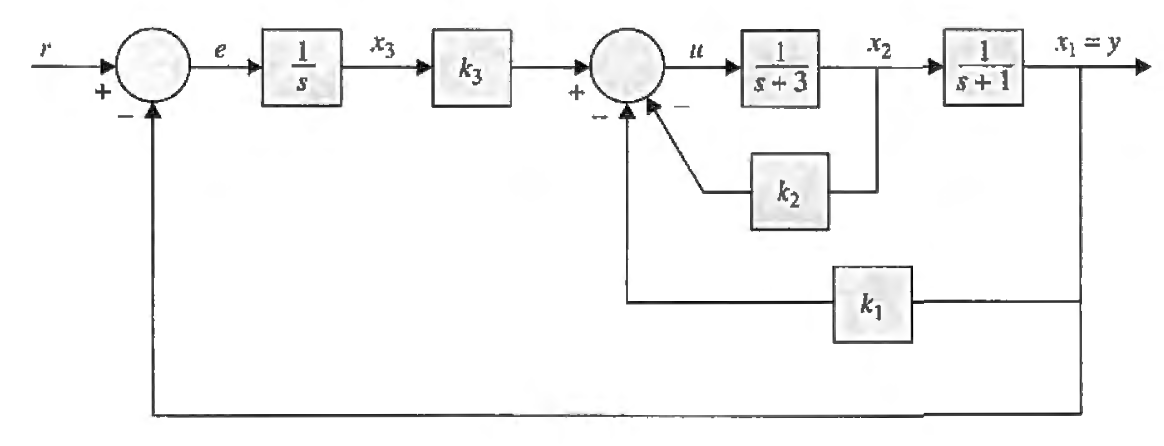
\includegraphics[width=\linewidth]{./figures/P10_59.png}
 \end{figure}

 \subsubsection*{(a) Find the values of the feedback gains so that:
 \begin{itemize}
    \item The steady-state error $e_{ss}$ [$e(t)$ is the error signal] due to a step input is zero.
    \item The characteristic equation roots are at $- 1+j$ , $-1-j$ , and $-10$.
\end{itemize}}

If we reduce the block diagram to a unity feedback system,
we get that the forward path transfer function, $G(s)$ is:

$$ G(s) = \frac{k_{3}}{s^3 + (k_{2} + 4) s^2 + (k_{1}+k_{2}+3)s} $$

The closed loop transfer function is:

$$ \frac{Y(s)}{R(s)} = \frac{G(s)}{1+G(s)}
= \frac{k_{3}}{s^3 + (k_{2} + 4) s^2 + (k_{1}+k_{2}+3)s + k_{3}}  $$

For $e_{ss}$ to be zero, when the input is a step function, $K_p$ must be infinite:

$$ K_p = \lim_{s \to 0} G(s) = \frac{k_{3}}{s^3 + (k_{2} + 4) s^2 + (k_{1}+k_{2}+3)s} = \infty $$

Since all values in the denominator multiply by $s$,
$\mathbf{e_{ss}}$ \textbf{is zero for all values of $\mathbf{k_1}$, $\mathbf{k_2}$, and $\mathbf{k_3}$} since:
\begin{answer}
$$ e_{ss} = \frac{R}{1+K_p} = \frac{R}{1+\infty} = 0 $$
\end{answer}

The characteristic equation is:

$$\text{CE: \ \ } s^3 + (k_{2} + 4) s^2 + (k_{1}+k_{2}+3)s + k_{3} = 0$$

And we want the characteristic equation roots to be  $- 1+j$ , $-1-j$ , and $-10$.
We make the following equivalence:

$$s^3 + (k_{2} + 4) s^2 + (k_{1}+k_{2}+3)s + k_{3} = s^3 + 12 s^2 + 22 s + 20 $$

If we equate like terms of $s$:

\begin{equation*}
    \begin{aligned}
        &(k_{2} + 4) = 12 &\rightarrow \ \ &k_{2} = 8\\
        &(k_{1}+k_{2}+3) = 22  &\rightarrow \ \  &k_{1} = 11\\
        &k_{3} = 20 &\rightarrow \ \  &k_{3} = 20
    \end{aligned}
\end{equation*}

\begin{answer}
Find the values of the feedback gains are:
\begin{equation*}
    \begin{aligned}
        &k_{1} = 11\\
        &k_{2} = 8\\
        &k_{3} = 20
    \end{aligned}
\end{equation*}

\end{answer}

% \color{white}
% \hspace*{6em}\inputminted[frame=leftline,fontsize=\footnotesize]{matlab}
% {./matlab/Problem_5_18.m}
% \color{black}

% \begin{figure}[H]
%     \centering
%     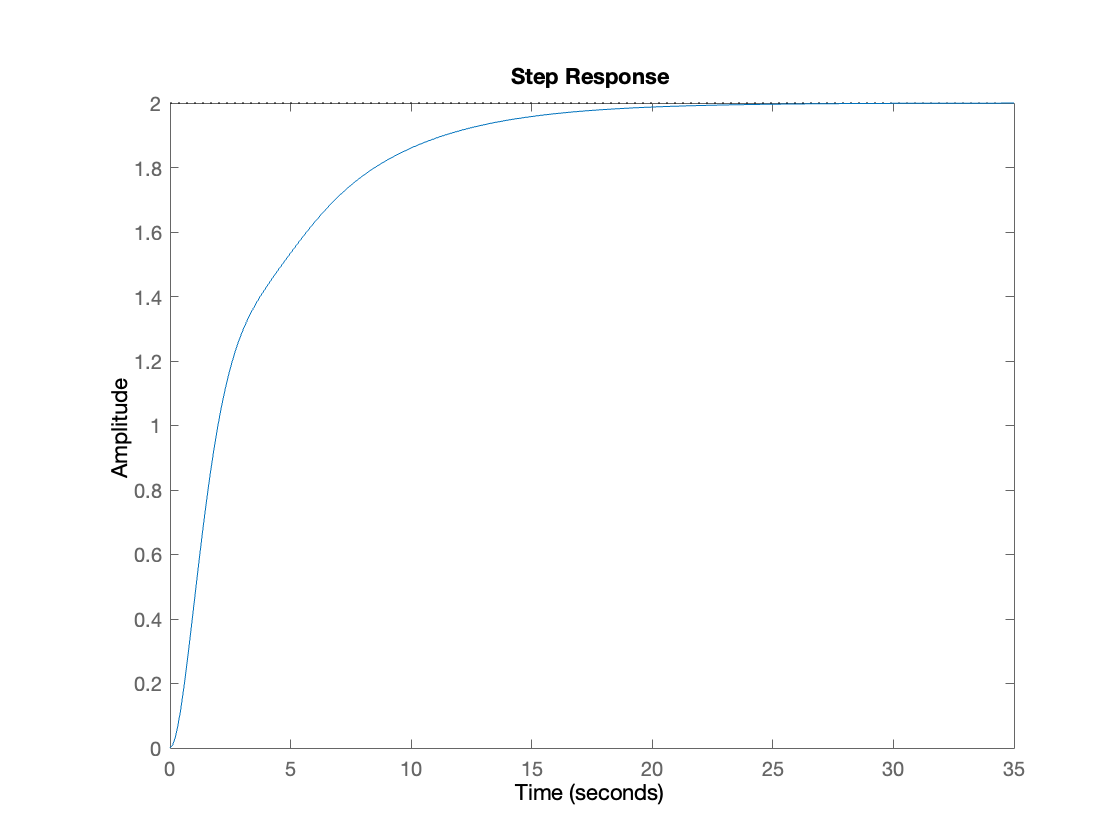
\includegraphics[width=0.7\linewidth]{./figures/step_response.png}
%     \caption{Step Response}
%     \label{fig:step}
%  \end{figure}



\end{document}

